\subsection{Debiased Contrastive Learning}\label{subsec:debiasing_cl}

\citet{chuang_debiased_2020} propose a debiased contrastive objective that corrects for sampling \acp{fn}, 
i.e., the selection of negative samples that have the same label as the anchor, in an unsupervised scenario.
They denote sampling bias the phenomenon where anchor $x$ and negative sample $x^-$ are similar to each other.
When randomly sampling negative samples from the data distribution $p(x)$ 
a negative sample can inherently belong to the same latent class as the anchor.

\begin{figure}%
    \centering
    \subfloat[\centering Visualization of sampling bias similar to \citet{chuang_debiased_2020}. Sampling $x_i^-$ from $p$ can result in \ac{fn}.]
    {{\includegraphics[width=5cm]{images/sampling_bias.png} }}%
    \qquad
    \subfloat[\centering Negative influence of sampling bias on accuracy from \citet{chuang_debiased_2020}.]{{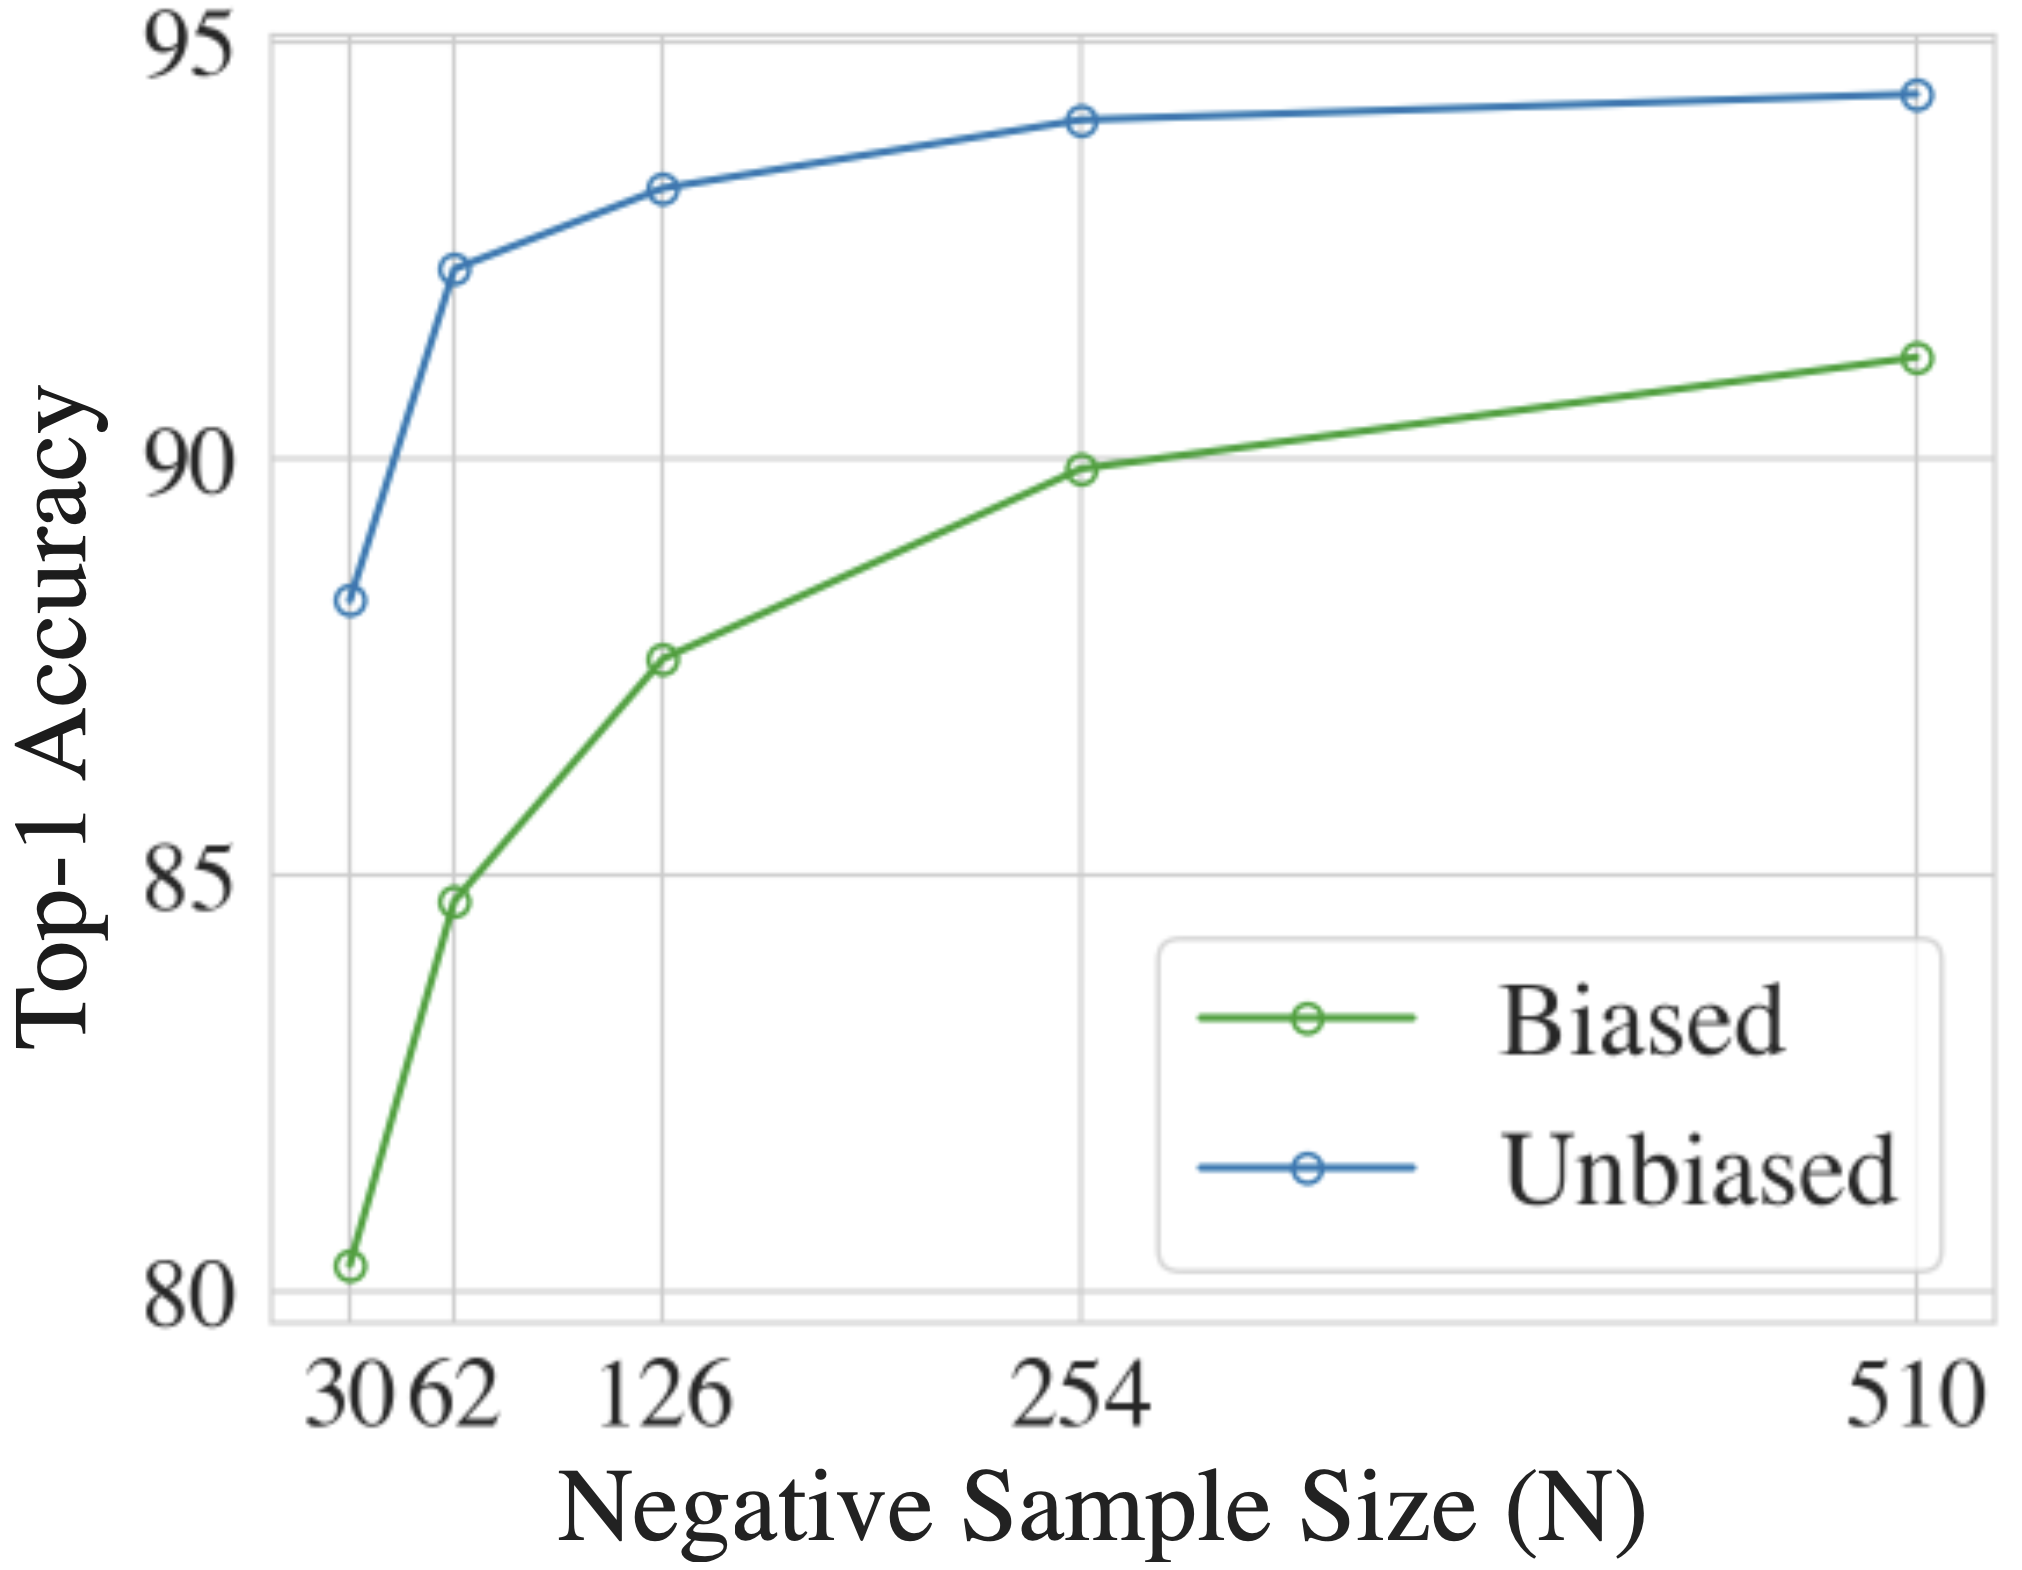
\includegraphics[width=5cm]{images/debiased_sampling_accuracy.png} }}%
    \caption{Visualization of sampling bias and its effect on the model's performance.}%
    \label{fig:sampling_bias}%
\end{figure}